The single asset test cases are designed to test the basic elements of the scenario risk calculator, such as:

\begin{itemize}
\item basic loss field computation
\item calculation of mean and standard deviation of scenario loss
\end{itemize}

\begin{table}

\centering
\begin{tabular}{ c l c c l }

\hline
\rowcolor{anti-flashwhite}
\bf{Site} & \bf{Taxonomy} & \bf{Latitude} & \bf{Longitude} & \bf{Comment} \\
\hline
1 & Wood & 38.113 & -122.000 & On fault midpoint, along strike \\
\hline
\end{tabular}

\caption{Asset location and taxonomy for the single-asset test cases}
\label{tab:asset}
\end{table}

The location and taxonomy of the single asset in the exposure model used for the single-asset test cases for the scenario risk calculator are given in Table \ref{tab:asset}.

% ---------------------------------------------------------------------------
\subsubsection{Case 1a}
Test Case~1a uses a set of five precomputed ground motion values to test the correct interpolation of the mean loss ratios of the vulnerability function at intermediate intensity measure levels. There is no uncertainty in the vulnerability function used for this case. The coefficient of variation of the loss ratio is zero at all intensity measure levels.

\begin{table}[htbp]

\centering
\begin{tabular}{ l c c l }

\hline
\rowcolor{anti-flashwhite}
\bf{GMF \#} & \bf{Site} & \bf{PGA (g)}\\
\hline
1 & 1 & 1.300 \\
2 & 1 & 0.044 \\
3 & 1 & 0.520 \\
4 & 1 & 1.000 \\
5 & 1 & 1.200 \\
\hline
\end{tabular}

\caption{Five precomputed ground motion fields at a single site}
\label{tab:gmfs-diff-l1-5}
\end{table}

Table~\ref{tab:gmfs-diff-l1-5} lists the five ground motion values used in this test case.

\begin{table}[htbp]

\centering
\begin{tabular}{ l c c c c c c c c c c c}

\hline
\rowcolor{anti-flashwhite}
\bf{PGA} & 0.05 & 0.20 & 0.40 & 0.60 & 0.80 & 1.00 & 1.20 & 1.40 & 1.60 & 1.80 & 2.00 \\
\hline
\bf{Mean LR} & 0.01 & 0.04 & 0.10 & 0.20 & 0.33 & 0.50 & 0.67 & 0.80 & 0.90 & 0.96 & 0.99 \\
\bf{CoV LR} & 0.0 & 0.0 & 0.0 & 0.0 & 0.0 & 0.0 & 0.0 & 0.0 & 0.0 & 0.0 & 0.0 \\
\hline
\end{tabular}

\caption{Vulnerability function with zero coefficients of variation}
\label{tab:vf-ln-tax1-zcov}
\end{table}

Table~\ref{tab:vf-ln-tax1-zcov} shows the mean loss ratios and corresponding coefficients of variation in the lognormal vulnerability function used in this test case. The vulnerability model is shown in Figure~\ref{fig:vf-ln-tax1-zcov}, where the dots represent the median loss ratios at a set of intensity levels.

\begin{figure}[htbp]
\centering
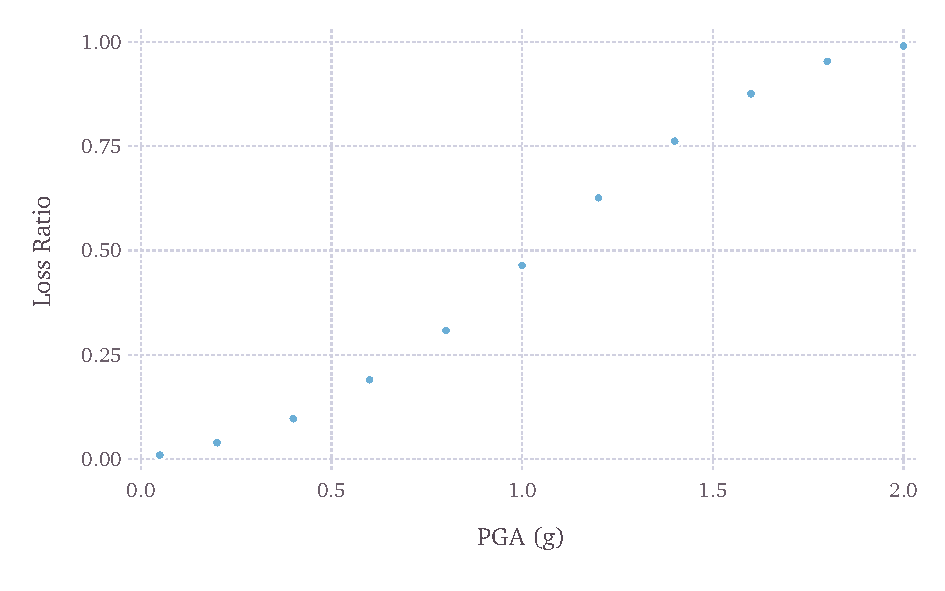
\includegraphics[width=12cm]{qareport/figures/fig-vf-ln-tax1-zcov}
\caption{Vulnerability model with zero coefficients of variation}
\label{fig:vf-ln-tax1-zcov}
\end{figure}

Since there is no variability in the loss ratio, calculation of the loss ratios is straightforward in this case. Since the coefficients of variation in the vulnerability function are all zero, the lognormal distribution devolves into the degenerate distribution. The ground motion values at the location of the single asset are $[1.3, 0.044, 0.52, 1.0, 1.2] g$. Consider the first value of $PGA = 1.3 g$. The vulnerability function for this case provides mean loss ratio values at intensity measure levels $1.2 g$ and $1.4 g$, but none at $1.3 g$. The mean loss ratios at $1.2 g$ and $1.4 g$ are $0.67$ and $0.80$ respectively.

The mean loss ratio at $1.3 g$ is obtained by interpolating between these two values. Linear interpolation gives a mean loss ratio of $0.735$ for $PGA = 1.3 g$.

Similar interpolation for the other ground motion values gives mean loss ratios of $0$, $0.16$, $0.5$, and $0.67$.

The mean loss ratio is simply obtained as the arithmetic mean of the five loss ratios as:

\begin{equation*}
\frac{0.735 + 0.0 + 0.16 + 0.50 + 0.67}{5} = 0.413
\end{equation*}

The standard deviation of the loss ratio is computed as:

\begin{multline*}
\sqrt{\frac{(0.735 - 0.413)^2 + (0.0 - 0.413)^2 + (0.16 - 0.413)^2 + (0.50 - 0.413)^2 + (0.67 - 0.413)^2}{5 - 1}} \\
= 0.320889
\end{multline*}

These numbers are multiplied by the asset value of $10,000$ to give the mean and standard deviation of loss for the scenario as $4,130$ and $3,208.89$ respectively.
\begin{table}[htbp]

\centering
\begin{tabular}{ l r r r }

\hline
\rowcolor{anti-flashwhite}
\bf{Result} & \bf{Expected} & \bf{OpenQuake} & \bf{Difference}\\
\hline
Mean loss & 4,130.00 & 4,130.00 & 0.00\% \\
Std. loss & 3,208.89 & 3,208.89 & 0.00\% \\
\hline
\end{tabular}

\caption{Results for scenario risk test case 1a}
\label{tab:result-sr-1a}
\end{table}
Table \ref{tab:result-sr-1a} shows the comparison of the OpenQuake result with the expected result.

% ---------------------------------------------------------------------------
\subsubsection{Case 1b}
This test case is identical to Case~1a described above, except for the use of the Beta CDF for the vulnerability functions instead of the lognormal CDF. Since the coefficients of variation in the vulnerability function are all zero, once again the Beta distribution devolves into the degenerate distribution as in the previous case. The results for this test case should be exactly the same as in Case~1a.
\begin{table}[htbp]

\centering
\begin{tabular}{ l r r r }

\hline
\rowcolor{anti-flashwhite}
\bf{Result} & \bf{Expected} & \bf{OpenQuake} & \bf{Difference}\\
\hline
Mean loss & 4,130.00 & 4,130.00 & 0.00\% \\
Std. loss & 3,208.89 & 3,208.89 & 0.00\% \\
\hline
\end{tabular}

\caption{Results for scenario risk test case 1b}
\label{tab:result-sr-1b}
\end{table}
Table \ref{tab:result-sr-1b} shows the comparison of the OpenQuake result with the expected result.

% ---------------------------------------------------------------------------
\subsubsection{Case 1c}
The purpose of this case is to test the correct sampling of the loss ratio from the prescribed distribution of the vulnerability function, given a specific intensity of ground motion. The 1,000 ground motion fields used in this test case are identical, i.e., variability in the ground motion is not considered in this case. However, in contrast to case 1a, variability in the loss ratio \emph{is} considered in the vulnerability function for this case. This permits us to compare the computed mean and standard deviation of the asset loss with the expected values, which are simply obtained through interpolation on the vulnerability function.

\begin{table}[htbp]

\centering
\begin{tabular}{ l c c l }

\hline
\rowcolor{anti-flashwhite}
\bf{GMF \#} & \bf{Site} & \bf{PGA (g)}\\
\hline
1 & 1 & 0.5000 \\
2 & 1 & 0.5000 \\
3 & 1 & 0.5000 \\
4 & 1 & 0.5000 \\
\vdots & \vdots & \vdots \\
1,000 & 1 & 0.5000 \\
\hline
\end{tabular}

\caption{1,000 identical ground motion fields at a single site}
\label{tab:gmfs-iden-l1-1000}
\end{table}

Table~\ref{tab:gmfs-iden-l1-1000} lists five of the one thousand identical ground motion values used in this test case.

\begin{table}[htbp]

\centering
\begin{tabular}{ l c c c c c c c c c c c}

\hline
\rowcolor{anti-flashwhite}
\bf{PGA} & 0.05 & 0.20 & 0.40 & 0.60 & 0.80 & 1.00 & 1.20 & 1.40 & 1.60 & 1.80 & 2.00 \\
\hline
\bf{Mean LR} & 0.01 & 0.04 & 0.10 & 0.20 & 0.33 & 0.50 & 0.67 & 0.80 & 0.90 & 0.96 & 0.99 \\
\bf{CoV LR} & 0.03 & 0.12 & 0.24 & 0.32 & 0.38 & 0.40 & 0.38 & 0.32 & 0.24 & 0.12 & 0.03 \\
\hline
\end{tabular}

\caption{Lognormal vulnerability function with nonzero coefficients of variation}
\label{tab:vf-ln-tax1-nzcov}
\end{table}

Table~\ref{tab:vf-ln-tax1-nzcov} shows the mean loss ratios and corresponding coefficients of variation in the vulnerability function used in this test case.

The vulnerability function for this case provides mean loss ratio values and coefficients of variation at intensity measure levels $PGA = 0.4 g$ and $0.6 g$, but none at $0.5 g$. Linear interpolation gives a mean loss ratio of $0.15$ for $PGA = 0.5 g$. Similarly, the coefficients of variation of the loss ratio at $0.4 g$ and $0.6 g$ are $0.24$ and $0.32$ respectively. The coefficient of variation of the loss ratio for $PGA = 0.5 g$ is obtained by linear interpolation as $0.28$.

The loss ratio at $PGA = 0.5 g$ follows a lognormal distribution with a mean of $0.15$ and a standard deviation of $0.28 \times 0.15 = 0.042$.

Since there is no variability in the ground motion, the expected value of the mean loss ratio for the scenario is also $0.15$, and the expected value of the standard deviation of the loss ratio is $0.042$.

These numbers are multiplied by the asset value of $10,000$ to give the expected mean and standard deviation of loss for the scenario as $1,500$ and $420$ respectively.

\begin{table}[htbp]

\centering
\begin{tabular}{ l r r r }

\hline
\rowcolor{anti-flashwhite}
\bf{Result} & \bf{Expected} & \bf{OpenQuake} & \bf{Difference}\\
\hline
Mean loss &  &  & \% \\
Std. loss &  &  & \% \\
\hline
\end{tabular}

\caption{Results for scenario risk test case 1c}
\label{tab:result-sr-1c}
\end{table}
Table \ref{tab:result-sr-1c} shows the comparison of the OpenQuake result with the expected result.

% ---------------------------------------------------------------------------
\subsubsection{Case 1d}
Test case 1d uses a set of 1,000 identical ground motion values, and described in Table \ref{tab:gmfs-iden-l1-1000}. However, in contrast to case 1a, variability in the loss ratio \emph{is} considered in the vulnerability function for this case.

\begin{table}[htbp]

\centering
\begin{tabular}{ l c c c c c c c c c c c}

\hline
\rowcolor{anti-flashwhite}
\bf{PGA} & 0.05 & 0.20 & 0.40 & 0.60 & 0.80 & 1.00 & 1.20 & 1.40 & 1.60 & 1.80 & 2.00 \\
\hline
\bf{Mean LR} & 0.01 & 0.04 & 0.10 & 0.20 & 0.33 & 0.50 & 0.67 & 0.80 & 0.90 & 0.96 & 0.99 \\
\bf{CoV LR} & 0.03 & 0.12 & 0.24 & 0.32 & 0.38 & 0.40 & 0.38 & 0.32 & 0.24 & 0.12 & 0.03 \\
\hline
\end{tabular}

\caption{Lognormal vulnerability function with nonzero coefficients of variation}
\label{tab:vf-ln-tax1-nzcov}
\end{table}

Table \ref{tab:vf-ln-tax1-nzcov} shows the mean loss ratios and corresponding coefficients of variation in the vulnerability function used in this test case.

Similar to case 1a described above, linear interpolation gives a mean loss ratio of $0.15$ for $PGA = 0.5 g$. The vulnerability function for this case provides coefficients of variation for the loss ratio at intensity measure levels $0.4 g$ and $0.6 g$, but none at $0.5 g$. The CoVs of the loss ratio at $0.4 g$ and $0.6 g$ are $0.24$ and $0.32$ respectively. The coefficient of variation of the loss ratio for $PGA = 0.5 g$ is thus obtained by linear interpolation as $0.28$.

The loss ratio at $PGA = 0.5 g$ follows a lognormal distribution with a mean of $0.15$ and a standard deviation of $0.28 \times 0.15 = 0.042$.

Since there is no variability in the ground motion, the mean loss ratio for the scenario is also $0.15$, and the standard deviation of the loss ratio is $0.042$.

These numbers are multiplied by the asset value of $10,000$ to give the mean and standard deviation of loss for the scenario as $1,500$ and $420$ respectively.
\begin{table}[htbp]

\centering
\begin{tabular}{ l r r r }

\hline
\rowcolor{anti-flashwhite}
\bf{Result} & \bf{Expected} & \bf{OpenQuake} & \bf{Difference}\\
\hline
Mean loss & 1,500.00 & 1,470.63 & 1.96\% \\
Std. loss & 420.00 & 1,345.84 & \textcolor{red}{-220.44\%} \\
\hline
\end{tabular}

\caption{Results for scenario risk test case 1d}
\label{tab:result-sr-1d}
\end{table}
Table \ref{tab:result-sr-1d} shows the comparison of the OpenQuake result with the expected result.

% ---------------------------------------------------------------------------
\subsubsection{Case 1e}
The purpose of this case is to test vulnerability functions that are specified as discrete probability mass functions rather than the parametric lognormal or beta distributions seen in the previous cases.

\begin{table}[htbp]

\centering
\begin{tabular}{ l c c c c c c c c c c c}

\hline
\rowcolor{anti-flashwhite}
\bf{LR | PGA} & \bf{0.05g} & \bf{0.20g} & \bf{0.40g} & \bf{0.60g} & \bf{1.00g} & \bf{1.40g} & \bf{1.60g} & \bf{2.00g} \\
\hline
\bf{0.000} & 0.995 & 0.950 & 0.490 & 0.300 & 0.140 & 0.030 & 0.010 & 0.004 \\
\bf{0.005} & 0.004 & 0.030 & 0.380 & 0.400 & 0.300 & 0.100 & 0.030 & 0.006 \\
\bf{0.050} & 0.001 & 0.015 & 0.080 & 0.160 & 0.240 & 0.300 & 0.100 & 0.010 \\
\bf{0.200} & 0.000 & 0.004 & 0.020 & 0.080 & 0.160 & 0.260 & 0.300 & 0.030 \\
\bf{0.450} & 0.000 & 0.001 & 0.015 & 0.030 & 0.100 & 0.180 & 0.300 & 0.180 \\
\bf{0.800} & 0.000 & 0.000 & 0.010 & 0.020 & 0.040 & 0.100 & 0.180 & 0.390 \\
\bf{1.000} & 0.000 & 0.000 & 0.005 & 0.010 & 0.020 & 0.030 & 0.080 & 0.380 \\
\hline
\end{tabular}

\caption{Vulnerability function specified using a discrete probability distribution. The values in each column specify the probability of occurrence of the corresponding loss ratio from the first column, for the ground motion intensity listed in the first row.}
\label{tab:vf-pm-tax1}
\end{table}



The vulnerability function used in this test case is shown in Table~\ref{tab:vf-pm-tax1}. This vulnerability function specifies a set of loss and the corresponding probabilities of occurrence for these loss ratios at different intensity measure levels.

The same identical ground motion values described earlier in Case~1c and shown in Table~\ref{tab:gmfs-iden-l1-1000} are used in this test case. However, the total number of ground motion fields is increased to 10,000 for this case, since the spread in the loss ratio distribution is much larger for the vulnerability function used in this case.

The vulnerability function for this case provides probabilities of occurrence for a set of loss ratios {0.000, 0.005, 0.050, 0.200, 0.450, 0.800, 1.000} at intensity measure levels $PGA = 0.4 g$ and $0.6 g$, but not at $0.5 g$. The specified set of probabilities for $PGA = 0.4 g$ are {0.490, 0.380, 0.080, 0.020, 0.015, 0.010, 0.005}, and those at $PGA = 0.6 g$ are {0.300, 0.400, 0.160, 0.080, 0.030, 0.020, 0.010}. Linear interpolation is used to obtain the probabilities of occurrence for the same set of loss ratios at $PGA = 0.5 g$ as {0.395, 0.390, 0.120, 0.050, 0.0225, 0.015, 0.0075}.

For the discrete random variable LR, which has the probability mass function (PMF): $lr_1 \mapsto p_1, \dotsc, lr_n \mapsto p_n$, the mean and standard deviation are calculated as:

\begin{equation}
\mu_{LR} = \sum_{i=1}^{n} p_i \cdot lr_i
\end{equation}

\begin{equation}
\sigma_{LR} = \sqrt{\sum_{i=1}^{n} p_i \cdot lr_i^2 - \mu_{LR}^2}
\end{equation}

Based on the above equations, the expected values of the mean and standard deviation of the loss ratio for our case are calculated as $0.047575$ and $0.147318$ respectively. These numbers are multiplied by the asset value of $10,000$ to give the expected mean and standard deviation of loss for the scenario as $475.75$ and $1,473.18$ respectively.
\begin{table}[htbp]

\centering
\begin{tabular}{ l r r r }

\hline
\rowcolor{anti-flashwhite}
\bf{Result} & \bf{Expected} & \bf{OpenQuake} & \bf{Difference}\\
\hline
Mean loss &  &  & \% \\
Std. loss &  &  & \% \\
\hline
\end{tabular}

\caption{Results for scenario risk test case 1e}
\label{tab:result-sr-1e}
\end{table}
Table \ref{tab:result-sr-1e} shows the comparison of the OpenQuake result with the expected result.

% ---------------------------------------------------------------------------
\subsubsection{Case 1f}
Variability in the ground motion is considered in all cases starting from Case~1f. Ten thousand ground motion fields are generated for the given rupture, taking into consideration both the inter-event and intra-event variability in the ground motion. The ground motion prediction equation used is Boore and Atkinson (2008).

The purpose of this case is to test the computation of the mean and standard deviation of the loss, given variability in both the ground motion values and in the lognormal vulnerability functions.

\begin{table}[htbp]

\centering
\begin{tabular}{ l c c l }

\hline
\rowcolor{anti-flashwhite}
\bf{GMF \#} & \bf{Site} & \bf{PGA (g)}\\
\hline
1 & 1 & 1.3495 \\
2 & 1 & 0.5393 \\
3 & 1 & 0.5240 \\
4 & 1 & 1.0385 \\
\vdots & \vdots & \vdots & \vdots \\
10,000 & 1 & 0.1327 \\
\hline
\end{tabular}

\caption{10,000 simulated ground motion fields}
\label{tab:gmfs-sim-l1-10000}
\end{table}

Table \ref{tab:gmfs-sim-l1-10000} lists five of the ten thousand ground motion values generated by OpenQuake.

Since the mean loss ratios in the vulnerability function are not a linear function of the intensity measure levels, an analytical solution for the mean and standard deviation of loss for the scenario cannot be found as in the previous cases. Thus, in order to check the OpenQuake results, an alternate implementation of the calculator algorithm in the programming language Julia is used for comparison. In order to provide a representative baseline for the comparison, one hundred thousand ground motion fields are used in the Julia calculation.

The mean and standard deviation of the logarithm of the ground motion calculated at the location of the asset as obtained by using the Boore and Atkinson (2008) equation are $-0.648$ and $0.564$ respectively. Assuming a lognormal distribution for the variability in the ground motion, ten thousand ground motion values are generated using Julia with these logarithmic mean and standard deviation values.

The mean loss ratio and standard deviation of loss ratio for each simulated ground motion value are obtained through interpolation on the mean loss ratios and corresponding coefficients of variation provided by the vulnerability function. Using the interpolated mean and standard deviation of loss ratios, one loss ratio is sampled for each ground motion value, assuming a lognormal distibution.

The mean and standard deviation of loss ratio for the scenario are estimated simply as the mean and standard deviation of the ten thousand simulated loss ratios.
\begin{table}[htbp]

\centering
\begin{tabular}{ l r r r }

\hline
\rowcolor{anti-flashwhite}
\bf{Result} & \bf{Julia} & \bf{OpenQuake} & \bf{Difference}\\
\hline
Mean loss & 2,404.92 & 2,370.74 & 1.42\% \\
Std. loss & 2,419.63 & 2,401.76 & 0.74\% \\
\hline
\end{tabular}

\caption{Results for scenario risk test case 1f}
\label{tab:result-sr-1f}
\end{table}

Table \ref{tab:result-sr-1f} shows the comparison of the OpenQuake result with the expected result.

% ---------------------------------------------------------------------------
\subsubsection{Case 1g}
This test case is identical to Case 1f described above, except for the use of the Beta CDF for the vulnerability functions instead of the lognormal CDF.
\begin{table}[htbp]

\centering
\begin{tabular}{ l r r r }

\hline
\rowcolor{anti-flashwhite}
\bf{Result} & \bf{Julia} & \bf{OpenQuake} & \bf{Difference}\\
\hline
Mean loss & 2,400.23 &  & \% \\
Std. loss & 2,417.74 &  & \% \\
\hline
\end{tabular}

\caption{Results for scenario risk test case 1g}
\label{tab:result-sr-1g}
\end{table}

Table \ref{tab:result-sr-1g} shows the comparison of the OpenQuake result with the expected result.

% ---------------------------------------------------------------------------
\subsubsection{Case 1h}
This test case repeats the exercise from Case~1f and Case~1g, using the discrete probability vulnerability functions instead of the parametric lognormal or Beta distribution based functions used in the previous two cases.

In this case, for each simulated ground motion value, the probabilities of occurrence of the set of loss ratios used by the vulnerability function are obtained through interpolation as described earlier in Case~1c. Using the set of loss ratios and the corresponding interpolated probabilities, one loss ratio is sampled for each ground motion value.

The mean and standard deviation of loss ratio for the scenario are estimated simply as the mean and standard deviation of the ten thousand simulated loss ratios. The OpenQuake values are compared with the alternate implementation of the algorithm in Julia.
\begin{table}[htbp]

\centering
\begin{tabular}{ l r r r }

\hline
\rowcolor{anti-flashwhite}
\bf{Result} & \bf{Expected} & \bf{OpenQuake} & \bf{Difference}\\
\hline
Mean loss &  &  & \% \\
Std. loss &  &  & \% \\
\hline
\end{tabular}

\caption{Results for scenario risk test case 1h}
\label{tab:result-sr-1h}
\end{table}
Table \ref{tab:result-sr-1h} shows the comparison of the OpenQuake result with the expected result.

% ---------------------------------------------------------------------------
\subsubsection{Case 2a}
In addition to computing direct structural losses, OpenQuake also provides support for computing losses incurred for the following other loss types:

\begin{itemize}
\item{Non-structural losses}
\item{Contents losses}
\item{Downtime, or business interruption losses}
\item{Occupant fatalities}
\end{itemize}

\begin{table}[htbp]

\centering
\begin{tabular}{ l c c c c c c c c c }

\hline
\rowcolor{anti-flashwhite}
\bf{PGA} & \bf{0.005g} & \bf{0.15g} & \bf{0.40g} & \bf{0.60g} & \bf{0.80g} & \bf{1.00g} & \bf{1.20g} & \bf{\dots} & \bf{2.00g} \\
\hline
\bf{Mean LR} & 0.01 & 0.05 & 0.12 & 0.24 & 0.40 & 0.60 & 0.80 & \dots & 1.00 \\
\bf{CoV LR} & 0.03 & 0.12 & 0.24 & 0.32 & 0.32 & 0.24 & 0.12 & \dots & 0.00 \\
\hline
\end{tabular}

\caption{Lognormal vulnerability function for non-structural components}
\label{tab:vf-ln-tax1-nst}
\end{table}
\begin{table}[htbp]

\centering
\begin{tabular}{ l c c c c c c c c c c c}

\hline
\rowcolor{anti-flashwhite}
\bf{PGA} & \bf{0.005g} & \bf{0.15g} & \bf{0.40g} & \bf{0.60g} & \bf{0.80g} & \bf{1.00g} & \bf{1.20g} & \bf{1.40g} & \bf{1.60g} & \bf{1.80g} & \bf{2.00g} \\
\hline
\bf{Mean LR} & 0.02 & 0.10 & 0.33 & 0.66 & 0.90 & 0.98 & 1.00 & 1.00 & 1.00 & 1.00 & 1.00 \\
\bf{CoV LR} & 0.03 & 0.12 & 0.24 & 0.24 & 0.12 & 0.03 & 0.00 & 0.00 & 0.00 & 0.00 & 0.00 \\
\hline
\end{tabular}

\caption{Lognormal vulnerability function for contents}
\label{tab:vf-ln-tax1-con}
\end{table}
\begin{table}[htbp]

\centering
\begin{tabular}{ l c c c c c c c c c c c}

\hline
\rowcolor{anti-flashwhite}
\bf{PGA} & \bf{0.005g} & \bf{0.15g} & \bf{0.40g} & \bf{0.60g} & \bf{0.80g} & \bf{1.00g} & \bf{1.20g} & \bf{\dots} & \bf{2.00g} \\
\hline
\bf{Mean LR} & 0.01 & 0.04 & 0.10 & 0.20 & 0.33 & 0.50 & 0.67 & \dots & 0.99 \\
\bf{CoV LR} & 0.03 & 0.12 & 0.24 & 0.32 & 0.38 & 0.40 & 0.38 & \dots & 0.03 \\
\hline
\end{tabular}

\caption{Lognormal vulnerability function for downtime}
\label{tab:vf-ln-tax1-dnt}
\end{table}
\begin{table}[htbp]

\centering
\begin{tabular}{ l c c c c c c c c c }

\hline
\rowcolor{anti-flashwhite}
\bf{PGA} & \bf{0.005g} & \bf{0.15g} & \bf{0.40g} & \bf{0.60g} & \bf{0.80g} & \bf{1.00g} & \bf{1.20g} & \bf{\dots} & \bf{2.00g} \\
\hline
\bf{Mean LR} & 0.0001 & 0.0004 & 0.0010 & 0.0020 & 0.0033 & 0.0050 & 0.0067 & \dots & 0.0099 \\
\bf{CoV LR} & 0.03 & 0.12 & 0.24 & 0.32 & 0.38 & 0.40 & 0.38 & \dots & 0.03 \\
\hline
\end{tabular}

\caption{Lognormal vulnerability function for occupants fatality}
\label{tab:vf-ln-tax1-occ}
\end{table}

The purpose of this case is to test the calculation of mean and standard deviation of non-structural losses for an asset. The replacement value of the non-structural components for the asset used in this case is $15,000$. Table~\ref{tab:vf-ln-tax1-nst} shows the mean loss ratios and corresponding coefficients of variation in the non-structural components vulnerability function used in this test case.
\begin{table}[htbp]

\centering
\begin{tabular}{ l r r r }

\hline
\rowcolor{anti-flashwhite}
\bf{Result} & \bf{Expected} & \bf{OpenQuake} & \bf{Difference}\\
\hline
Mean loss &  &  & \% \\
Std. loss &  &  & \% \\
\hline
\end{tabular}

\caption{Results for scenario risk test case 2a}
\label{tab:result-sr-2a}
\end{table}
Table \ref{tab:result-sr-2a} shows the comparison of the OpenQuake result with the expected result.

% ---------------------------------------------------------------------------
\subsubsection{Case 2b}
The purpose of this case is to test the calculation of mean and standard deviation of the contents losses for an asset. The replacement value of the contents for the asset used in this case is $5,000$. Table~\ref{tab:vf-ln-tax1-con} shows the mean loss ratios and corresponding coefficients of variation in the contents vulnerability function used in this test case.
\begin{table}[htbp]

\centering
\begin{tabular}{ l r r r }

\hline
\rowcolor{anti-flashwhite}
\bf{Result} & \bf{Expected} & \bf{OpenQuake} & \bf{Difference}\\
\hline
Mean loss &  &  & \% \\
Std. loss &  &  & \% \\
\hline
\end{tabular}

\caption{Results for scenario risk test case 2b}
\label{tab:result-sr-2b}
\end{table}
Table \ref{tab:result-sr-2b} shows the comparison of the OpenQuake result with the expected result.

% ---------------------------------------------------------------------------
\subsubsection{Case 2c}
The purpose of this case is to test the calculation of mean and standard deviation of downtime, or business-interruption losses for an asset. The loss due to downtime, or business-interruption for the asset used in this case is $2,000 / month$. Downtime losses are usually specified per unit time the asset will be unavailable for occupancy or use. Table~\ref{tab:vf-ln-tax1-dnt} shows the mean loss ratios and corresponding coefficients of variation for the downtime vulnerability function used in this test case.
\begin{table}[htbp]

\centering
\begin{tabular}{ l r r r }

\hline
\rowcolor{anti-flashwhite}
\bf{Result} & \bf{Expected} & \bf{OpenQuake} & \bf{Difference}\\
\hline
Mean loss &  &  & \% \\
Std. loss &  &  & \% \\
\hline
\end{tabular}

\caption{Results for scenario risk test case 2c}
\label{tab:result-sr-2c}
\end{table}
Table \ref{tab:result-sr-2c} shows the comparison of the OpenQuake result with the expected result.

% ---------------------------------------------------------------------------
\subsubsection{Case 2d}
The purpose of this case is to test the calculation of mean and standard deviation of occupant fatalities for an asset. The number of occupants for the asset used in this case are 2 (day), 4 (transit), and 6 (night). Table~\ref{tab:vf-ln-tax1-dnt} shows the mean loss ratios and corresponding coefficients of variation for the occupants fatality vulnerability function used in this test case.
\begin{table}[htbp]

\centering
\begin{tabular}{ l r r r }

\hline
\rowcolor{anti-flashwhite}
\bf{Result} & \bf{Julia} & \bf{OpenQuake} & \bf{Difference}\\
\hline
Mean loss & 1.45 \times 10^{-2} & 9.56 \times 10^{-3} & \textcolor{red}{34.12\%} \\
Std. loss & 1.44 \times 10^{-2} & 9.55 \times 10^{-3} & \textcolor{red}{33.80\%} \\
\hline
\end{tabular}

\caption{Results for scenario risk test case 2d}
\label{tab:result-sr-2d}
\end{table}

Table \ref{tab:result-sr-2d} shows the comparison of the OpenQuake result with the expected result.


% ---------------------------------------------------------------------------
\subsubsection{Case 3a}
There are several ways by which the replacement value of an asset can be specified in the exposure model. The different options are listed below:

\begin{itemize}
	\item Specify the aggregate value of each asset
	\item Specify the value per unit, and provide the number of units in each asset
	\item Specify the value per unit area, and provide the aggregate area of each asset
	\item Specify the value per unit area, specify the area per unit, and provide the number of units in each asset
\end{itemize}

This case tests the computation of the mean and standard deviation of the loss when the aggregate asset value is provided in the exposure model. The vulnerability function used is the same as in Case~1f and shown in Table~\ref{tab:vf-ln-tax1-nzcov}. The aggregate asset value in this case is $20,000$.
\begin{table}[htbp]

\centering
\begin{tabular}{ l r r r }

\hline
\rowcolor{anti-flashwhite}
\bf{Result} & \bf{Julia} & \bf{OpenQuake} & \bf{Difference}\\
\hline
Mean loss & 4,809.84 & 4,741.48 & 1.42\% \\
Std. loss & 4,839.26 & 4,803.54 & 0.74\% \\
\hline
\end{tabular}

\caption{Results for scenario risk test case 3a}
\label{tab:result-sr-3a}
\end{table}
Table \ref{tab:result-sr-3a} shows the comparison of the OpenQuake result with the expected result.

% ---------------------------------------------------------------------------
\subsubsection{Case 3b}
This case tests the computation of the mean and standard deviation of the loss when the value of the assets is specified per unit, and the number of units in each asset are provided in the exposure model. The vulnerability function used is the same as in Case~1f and shown in Table~\ref{tab:vf-ln-tax1-nzcov}. The asset has two units, and the value per unit is $7,500$. The aggregate asset value in this case is $15,000$.
\begin{table}[htbp]

\centering
\begin{tabular}{ l r r r }

\hline
\rowcolor{anti-flashwhite}
\bf{Result} & \bf{Julia} & \bf{OpenQuake} & \bf{Difference}\\
\hline
Mean loss & 3,607.38 & 3,556.11 & 1.42\% \\
Std. loss & 3,629.45 & 3,602.65 & 0.74\% \\
\hline
\end{tabular}

\caption{Results for scenario risk test case 3b}
\label{tab:result-sr-3b}
\end{table}
Table \ref{tab:result-sr-3b} shows the comparison of the OpenQuake result with the expected result.
% ---------------------------------------------------------------------------
\subsubsection{Case 3c}
This case tests the computation of the mean and standard deviation of the loss when the value of the assets is specified per unit area, and the aggregate area of each asset is provided in the exposure model. The vulnerability function used is the same as in Case~1f and shown in Table~\ref{tab:vf-ln-tax1-nzcov}. The asset has an aggregate area of $1,000$ sq. units, and the value per unit area is $5$. The aggregate asset value in this case is $5,000$.
\begin{table}[h]

\centering
\begin{tabular}{ l r r r }

\hline
\rowcolor{anti-flashwhite}
\bf{Result} & \bf{Julia} & \bf{OpenQuake} & \bf{Difference}\\
\hline
Mean loss & 1,202.46 & 1,185.37 & 1.42\% \\
Std. loss & 1,209.82 & 1,200.88 & 0.74\% \\
\hline
\end{tabular}

\caption{Results for scenario risk test case 3c}
\label{tab:result-sr-3c}
\end{table}
Table \ref{tab:result-sr-3c} shows the comparison of the OpenQuake result with the expected result.

% ---------------------------------------------------------------------------
\subsubsection{Case 3d}
This case tests the computation of the mean and standard deviation of the loss when the value of the assets is specified per unit area, the area is specified per unit, and the number of units in each asset are provided in the exposure model. The vulnerability function used is the same as in Case~1f and shown in Table~\ref{tab:vf-ln-tax1-nzcov}. The asset has three units, the area per unit is $400$ sq. units, and the value per unit area is $10$. The aggregate asset value in this case is $12,000$.
\begin{table}[h]

\centering
\begin{tabular}{ l r r r }

\hline
\rowcolor{anti-flashwhite}
\bf{Result} & \bf{Julia} & \bf{OpenQuake} & \bf{Difference}\\
\hline
Mean loss & 2,885.90 & 2,844.89 & 1.42\% \\
Std. loss & 2,903.56 & 2,882.12 & 0.74\% \\
\hline
\end{tabular}

\caption{Results for scenario risk test case 3d}
\label{tab:result-sr-3d}
\end{table}
Table \ref{tab:result-sr-3d} shows the comparison of the OpenQuake result with the expected result.
